\section{Details of benchmark sequences}
\label{app-mask:d}
\newcolumntype{D}{>{\centering\arraybackslash}p{13.2cm}}
\setlength{\tabcolsep}{12pt}
\begin{table}[h]
\begin{center}
\begin{tabular}{lll} 
    \toprule
    Label & Description (Assembly) & Length \\
    \midrule
    \textsc{ChrXC} & Centromere region of human chromosome X \cite{miga19} & 3106132 \\ 
    \textsc{Chr1} & Human chromosome 1 & 233587144 \\ 
    \textsc{Btr1} & Blautia producta (GCA\_004210255.1) & 6354838 \\ 
    \textsc{Btr2} & Blautia hansenii DSM 20583 (GCF\_002222595.2) & 3065949 \\ 
    \textsc{Btr3} & [Clostridium] scindens (GCA\_009684695.1) & 3785527 \\ 
    \textsc{Btr4} & Blautia producta ATCC 27340 = DSM 2950 (GCA\_010669205.1) & 6197116 \\ 
    \bottomrule
\end{tabular}
\end{center}
\caption{Descriptions and lengths of sequences used in Section~\ref{sec:result}.}
\label{table:4}
\end{table}

\section{Other implementation details}
\label{app-mask:e}
We implement our method using PyTorch and deploy all experiments on a
RTX-3080 GPU. Due to limited GPU memory, each training epoch only computes the loss on a randomly sampled batch of $32$ substrings of length $\ell = 1500$ bases. The conservation component of $\mathcal{L}_{gss}$ is averaged over $5$ random mutations, simulated using a $10\%$ base substitution rate. Evaluation of conservation is likewise obtained using $5$ random mutations. Network weights are optimized using the ADAM optimizer \cite{kingma14adam} with default parameters.

\section{Other results}
\label{app-mask:f}
\subsubsection{Effectiveness of training on conservation and density metrics.} Fig.~\ref{fig:5} demonstrates the individual effect of training the proposed loss $\mathcal{L}_{gss}$ on the conservation and density metrics. We observe that both conservation and density of the syncmer mask are upper-bounded by that of the minimizer mask, which confirms the result of  Theorem~\ref{theo:1}. We observe that $\mathcal{L}_{gss}$ improves conservation but worsens density for the syncmer mask, which is similar to our first experiment. However, this is not the case for the minimizer and complement mask, which obtain significant improvements in both metrics over $600$ training epochs. We note that this does not contradict our analysis, as conservation is still bounded by density at any point during the training. Rather, this implies that our method has found a favorable trade-off between the two metrics, which in turn explains the sharper increases in GSS compared to that of syncmer across all experiments.

\begin{figure}[ht]
\centering
\begin{tabular}{cc}
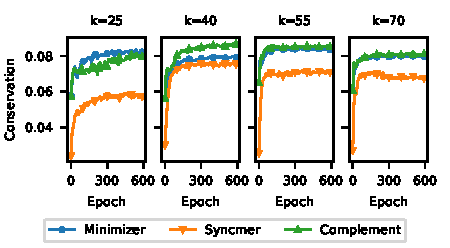
\includegraphics[scale=1]{masked_mnz_plots/fig5/compare_con_vs_epoch_chrXC.pdf} & 
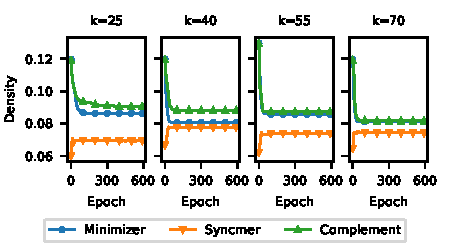
\includegraphics[scale=1]{masked_mnz_plots/fig5/compare_den_vs_epoch_chrXC.pdf} \end{tabular}  
\caption{Comparing conservation and density metrics of different masked minimizers vs.\@ number of training epochs on \textsc{ChrXC} with $w=15$ and $k\in\{25,40,55,70\}$.}
\label{fig:5}
\end{figure}

\subsubsection{GSS profiles of minimizer masks on other bacterial genomes.} Fig.~\ref{fig:4b} shows the scatter plots of all $2^w$ masked minimizers trained on \textsc{Btr1}, \textsc{Btr2} and \textsc{Btr3} using $\mathcal{L}_{gss}$ with $w=10$ and $k=15$, grouped by the number of $1$-entries in their masks. We observe the same increasing pattern of average GSS with respect to number of $1$-entries in the mask, thus confirming that the minimizer mask is indeed a good default choice.

\begin{figure}[ht]
\centering
\begin{tabular}{c}
\hspace{-3mm}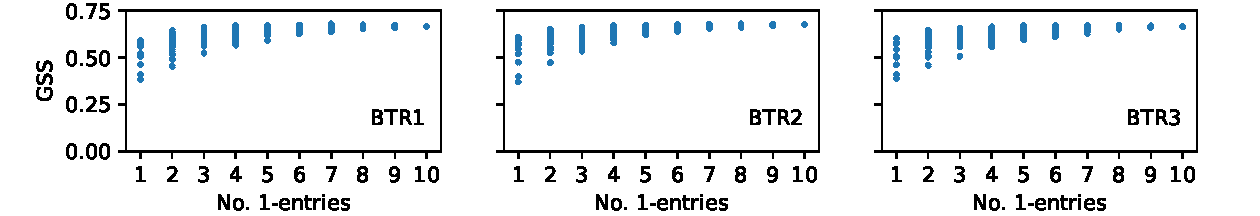
\includegraphics[scale=0.78]{masked_mnz_plots/fig4/exp7b.pdf}
\end{tabular}
\caption{GSS vs.\@ number of $1$-entries of all mask minimizers on bacterial genomes \textsc{Btr1-3}.}
\label{fig:4b}
\end{figure}

\subsubsection{Exploiting the relative conservation metric with varying offsets.} We repeat this experiment for different syncmer masks with $t\in\{6,7,8,9\}$ and plot all results in Fig.~\ref{fig:6}. In all of these experiments, we observe that the model trained with $n=20$ sampled mutations per epoch always find the exploit within $1000-1500$ epochs. The bar plots once again confirm that for each value of $t$, the exploitative solution contains no segment with more than $t-1$ consecutively decreasing scores. We note that the total count for $t=7$ is significantly lower than other values of $t$ because the solution contains several segments of monotonically increasing scores that are relatively long, which count towards the $>6$ bucket.

\begin{figure}[ht]
\centering
\begin{tabular}{c}
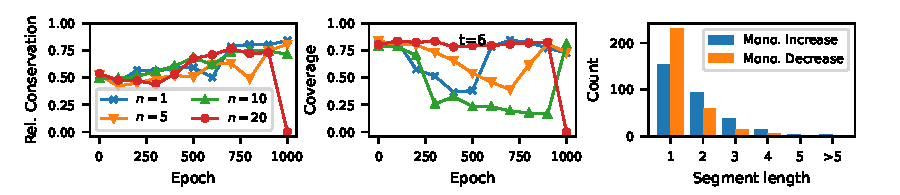
\includegraphics[scale=1.075]{masked_mnz_plots/fig6/exploit_t6.pdf} \\
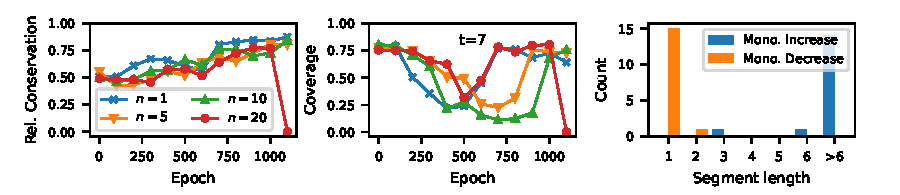
\includegraphics[scale=1.075]{masked_mnz_plots/fig6/exploit_t7.pdf} \\
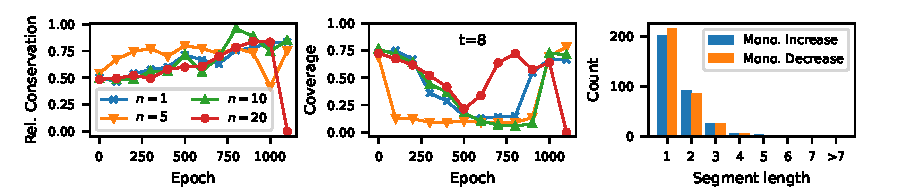
\includegraphics[scale=1.075]{masked_mnz_plots/fig6/exploit_t8.pdf} \\
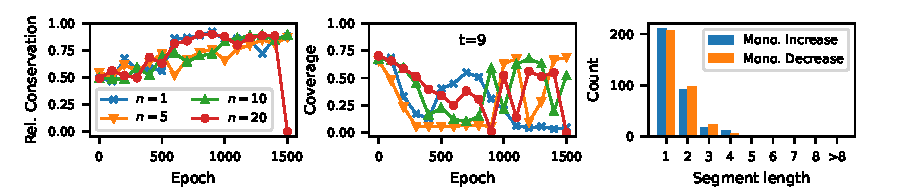
\includegraphics[scale=1.075]{masked_mnz_plots/fig6/exploit_t9.pdf} \\
\end{tabular}
\caption{Finding the relative conservation exploit for various syncmer masks with (from top to bottom) offset $t \in \{6,7,8,9\}$ with $\mathcal{L}_{exploit}$, $w=10$ and $k=15$.}
\label{fig:6}
\end{figure}